\documentclass[a4]{article}
\pagestyle{myheadings}

%%%%%%%%%%%%%%%%%%%
% Packages/Macros %
%%%%%%%%%%%%%%%%%%%
\usepackage{mathrsfs}


\usepackage{fancyhdr}
\pagestyle{fancy}
\lhead{}
\chead{}
\rhead{}
\lfoot{}
\cfoot{} 
\rfoot{\normalsize\thepage}
\renewcommand{\headrulewidth}{0pt}
\renewcommand{\footrulewidth}{0pt}
\newcommand{\RomanNumeralCaps}[1]
{\MakeUppercase{\romannumeral #1}}

\usepackage{amssymb,latexsym}  % Standard packages
\usepackage[utf8]{inputenc}
\usepackage[russian]{babel}
\usepackage{MnSymbol}
\usepackage{amsmath,amsthm}
\usepackage{indentfirst}
\usepackage{graphicx}%,vmargin}
\usepackage{graphicx}
\graphicspath{{pictures/}} 
\usepackage{verbatim}
\usepackage{color}









\DeclareGraphicsExtensions{.pdf,.png,.jpg}% -- настройка картинок

\usepackage{epigraph} %%% to make inspirational quotes.
\usepackage[all]{xy} %for XyPic'a
\usepackage{color} 
\usepackage{amscd} %для коммутативных диграмм


\newtheorem{Lemma}{Лемма}[section]
\newtheorem{Proposition}{Предложение}[section]
\newtheorem{Theorem}{Теорема}[section]
\newtheorem{Corollary}{Следствие}[section]
\newtheorem{Remark}{Замечание}[section]
\newtheorem{Definition}{Определение}[section]
\newtheorem{Designations}{Обозначение}[section]




%%%%%%%%%%%%%%%%%%%%%%%% 
%Сношение с оглавлением% 
%%%%%%%%%%%%%%%%%%%%%%%% 
\usepackage{tocloft} 
\renewcommand{\cftdotsep}{2} %частота точек
\renewcommand\cftsecleader{\cftdotfill{\cftdotsep}}
\renewcommand{\cfttoctitlefont}{\hspace{0.38\textwidth} \LARGE\bfseries} 
\renewcommand{\cftsecaftersnum}{.}
\renewcommand{\cftsubsecaftersnum}{.}
\renewcommand{\cftbeforetoctitleskip}{-1em} 
\renewcommand{\cftaftertoctitle}{\mbox{}\hfill \\ \mbox{}\hfill{\footnotesize Стр.}\vspace{-0.5em}} 
\renewcommand{\cftsubsecfont}{\hspace{1pt}} 
\renewcommand{\cftparskip}{3mm} %определяет величину отступа в оглавлении
\setcounter{tocdepth}{5} 




\addtolength{\textwidth}{0.7in}
\textheight=630pt
\addtolength{\evensidemargin}{-0.4in}
\addtolength{\oddsidemargin}{-0.4in}
\addtolength{\topmargin}{-0.4in}

\newcommand{\empline}{\mbox{}\newline} 
\newcommand{\likechapterheading}[1]{ 
	\begin{center} 
		\textbf{\MakeUppercase{#1}} 
	\end{center} 
	\empline} 

\makeatletter 
\renewcommand{\@dotsep}{2} 
\newcommand{\l@likechapter}[2]{{\bfseries\@dottedtocline{0}{0pt}{0pt}{#1}{#2}}} 
\makeatother 
\newcommand{\likechapter}[1]{ 
	\likechapterheading{#1} 
	\addcontentsline{toc}{likechapter}{\MakeUppercase{#1}}} 





\usepackage{xcolor}
\usepackage{hyperref}
\definecolor{linkcolor}{HTML}{000000} % цвет ссылок
\definecolor{urlcolor}{HTML}{AA1622} % цвет гиперссылок

\hypersetup{pdfstartview=FitH,  linkcolor=linkcolor,urlcolor=urlcolor, colorlinks=true}



\def \newstr {\medskip \par \noindent} 



\begin{document}
	\def\contentsname{\LARGE{Содержание}}
	\thispagestyle{empty}
	\begin{center} 
		\vspace{2cm} 
		{\Large \sc Санкт-Петербургский Политехнический Университет}\\
		\vspace{2mm}
		{\Large\sc Петра Великого}\\
		\vspace{1cm}
		{\large \sc Институт прикладной математики и механики\\ 
			\vspace{0.5mm}
			\textsc{}}\\ 
		\vspace{0.5mm}
		{\large\sc Кафедра $"$Прикладная математика$"$}\\
		\vspace{15mm}
		
		
		{\sc \textbf{Отчёт\\
			Лабораторная работа №$4$\\
			по дисциплине\\
			"Математическая статистика"}
			\vspace{6mm}
			
		}
		\vspace*{2mm}
		
		
		\begin{flushleft}
			\vspace{4cm}
			\sc Выполнил студент:\\
			\sc Салихов С.Р.\\
			\sc группа: 3630102/70401\\
			\vspace{1cm}
			\sc Проверил:\\
			\sc к.ф-м.н., доцент\\
			\sc Баженов Александр Николавич
			\vspace{20mm}
		\end{flushleft}
	\end{center} 
	\begin{center}
		\vfill {\large\textsc{Санкт-Петербург}}\\ 
		2020 г.
	\end{center}
	
	\newpage
	\pagestyle{plain}
	
	%\begin{center}
	%\begin{abstract} 
	
	%\end{abstract}
	
	%\end{center}
	
	\newpage
	\tableofcontents{}
	\newpage
	\listoffigures
	\newpage
	\listoftables
	\newpage
	
	
	\section{Постановка задачи}
	
	Для 5-ти рапределений:\\
		Нормальное распределение $N(x,0,1)$\\
		Распределение Коши $C(x,0,1)$\\
		Распределение Лапласа $L( x,0,\frac{1}{\sqrt{2}})$\\
		Распределение Пуассона $P(k, 10)$\\
		Равномерное Распределение $U(x,-\sqrt{3}, \sqrt{3})$\\
		
		Сгенерировать выборки размером 20, 60, и 100 элементов.\\
		Построить на них эмпирические функции распределения и ядерные
		оценки плотности распределения на отрезке $[-4; 4]$ для непрерывных
		распределений и на отрезке [6; 14] для распределения Пуассона.
		
	
	\section{Теория}
		\subsection{Эмпирическая функция распределения}
			\subsubsection{Статистический ряд}
				Статистическим рядом называется последовательность различных элементов выборки$ z_1, ... , z_k$, расположенных в возрастающем порядке с указанием частот $n_1, ... , n_k$, с которыми эти элементы содержатся в выборке.
				Статистический ряд обычно записывается в виде таблицы.
			\subsubsection{Определение}
				Эмпирической (выборочной) функцией распределения (э. ф. р.) называется
				относительная частота события $X < x$, полученная по данной выборке:
				$$F^*_n(x) = P^*(X<x)$$.
			\subsubsection{Описание}
				Для получения относительной частоты $P^*(X<x)$ просуммируем в статистическом ряде, построенном по данной выборке, все частоты $n_i$ , для
				которых элементы $z_i$ статистического ряда меньше x. Тогда $P^*(X<x) = \frac{1}{n}\sum_{z_i<x}n_i $. Получаем\\
				$$F^*(x) = \frac{1}{n}\sum_{z_i<x}n_i$$
				$F^*$(x) — функция распределения дискретной случайной величины $X^*$
				, заданной таблицей распределения.
				Эмпирическая функция распределения является оценкой, т. е. приближённым значением, генеральной функции распределения.
				$$F^*_n(x) \approx F_X(x)$$
				
		\subsection{Оценки плотности вероятности}
			\subsubsection{Определение}
				Оценкой плотности вероятности f(x) называется функция $\hat{f}$(x), построенная на основе выборки, приближенно равная f(x) $$\hat{f}(x) \approx f(x)$$
			\subsubsection{Ядерные оценки}
			ёПредставим оценку в виде суммы с числом слагаемых, равным объёму выборки: 
			$$\hat{f_n}(x) = \frac{1}{n h_n} \sum_{i = 1}^{n} K(\frac{x - x_i}{h_n})$$
			Здесь функция K(u), называемая ядерной (ядром), непрерывна и является плотностью вер-ти, $x_1, ..., x_n$ - элементы выборки, {$h_n$} - любая последовательноть положительных чисел, обладающая свойствами:\\
			1)при n-> $\infty$ $h_n$->0\\
			2)$\frac{h_n}{n^{-1}}$ -> $\infty$ ,когда n->$\infty$.\\
			Такие оценки называются непрерывными ядерными.\\
			
			Замечание. Свойство, означающее сближение оценки с оцениваемой величиной при n -> $\infty$ в каком-либо смысле, называется состоятельностью оценки.\\
			Если плотность f(x) кусочно-непрерывная, то ядерная оценка плотности
			является состоятельной при соблюдении условий, накладываемых на параметр сглаживания $h_n$, а также на ядро K(u).\\
			Гауссово(нормальное) ядро$$K(u) = \frac{1}{\sqrt{2 \pi}} e^{-\frac{u^2}{2}}$$
			Правило Сильвермана
			 $$h_n = 1.06 \hat{\sigma} n^{-0.2}$$, где $\hat{\sigma}$ - выборочное среднее отклонение.
		
	\section{Реализация}
	Для генерации выборки был использован $Python\;3.7$: модуль $random$ библиотеки $numpy$ для генерации случайных чисел с различными распределениями. Графики построены средствами matplotlib.
	\newpage
	\section{Результаты}
		\subsection{Эмпирическая функция распределений}
		Красный график - эталонная функция. Синий график - эмпирическая соответственно.
		\begin{center}
			
			\begin{figure}[h!]
				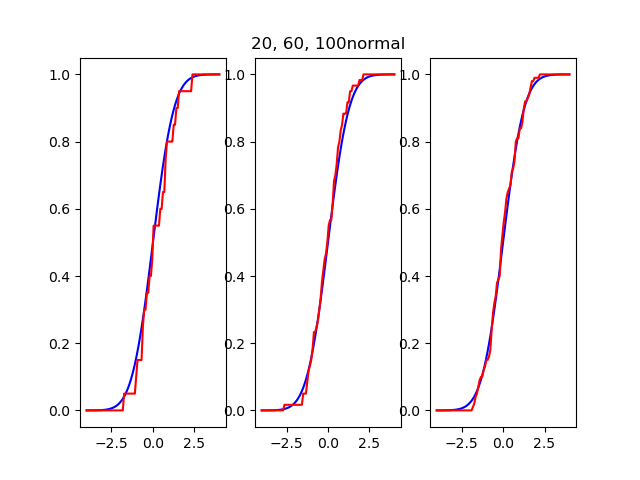
\includegraphics[width=\textwidth]{normalemp.png} 
				\caption[Нормальное распределение]{Нормальное распределение}
			\end{figure}
			\newpage
			\begin{figure}[h!]
				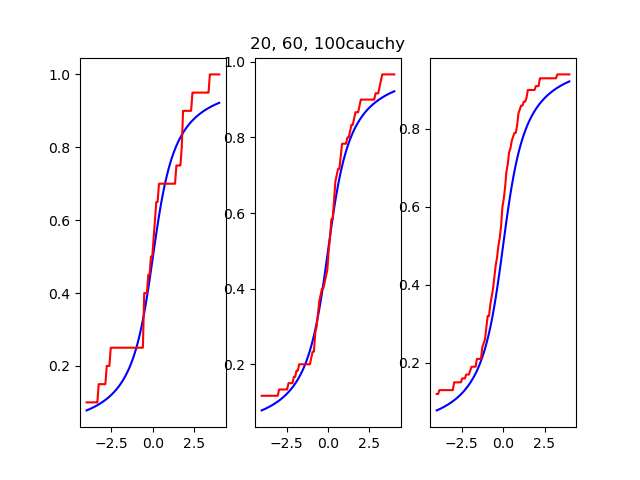
\includegraphics[width=\textwidth]{cauchyemp.png}
				\caption[Распределение Коши]{Распределение Коши}
			\end{figure}
			\newpage
			\begin{figure}[h!]
				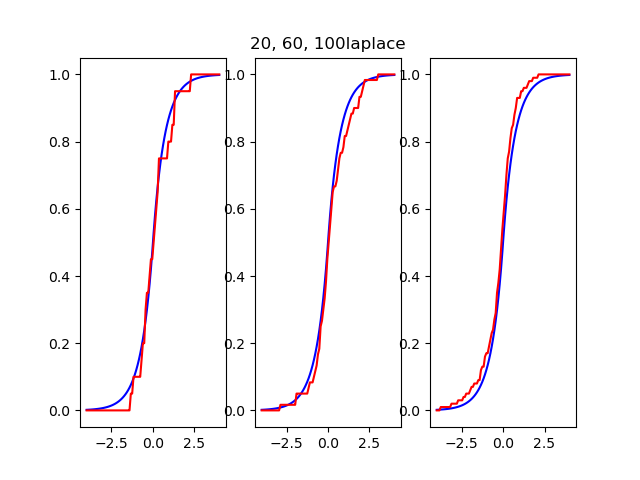
\includegraphics[width=\textwidth]{laplaceemp.png}
				\caption[Распределение Лапласа]{Распределение Лапласа}
			\end{figure}
			\newpage
			\begin{figure}[h!]
				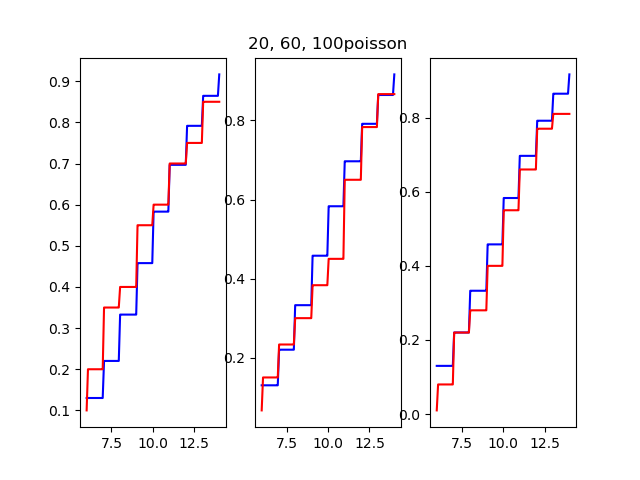
\includegraphics[width=\textwidth]{poissonemp.png}
				\caption[Распределение Пуассона]{Распределение Пуассона}
			\end{figure}
			\newpage
			\begin{figure}[h!]
				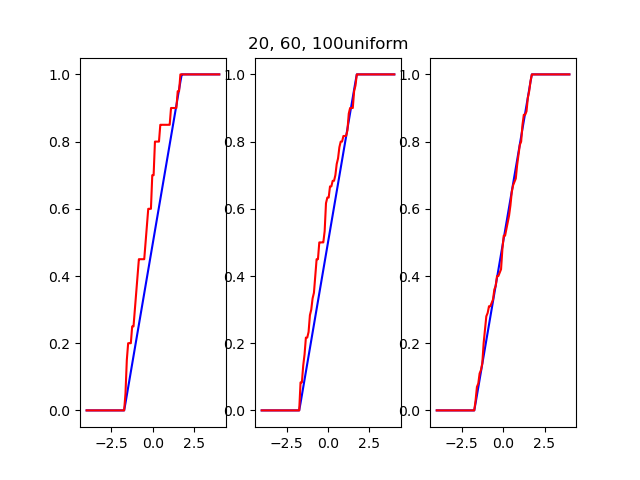
\includegraphics[width=\textwidth]{uniformemp.png}
				\caption[Равномерное распределение]{Равномерное распределение}
			\end{figure}
		\newpage
			
		\end{center}
		\subsection{Ядерные оценки плотности распределений}
		Черный цвет - эталонная функция. Красный цвет - эмпирическая.
		\begin{center}
		\begin{figure}[h!]
			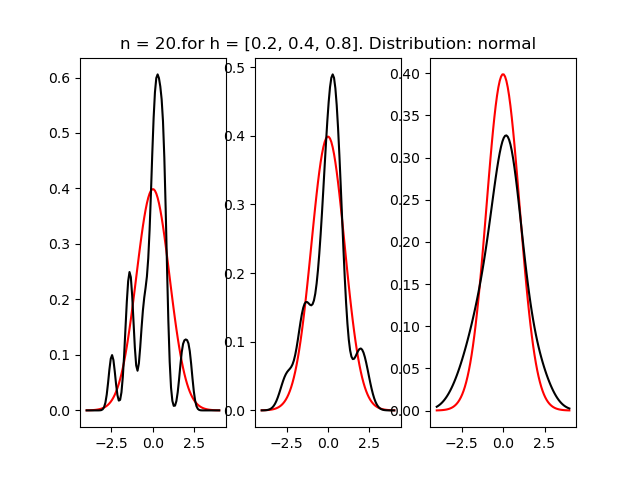
\includegraphics[width=\textwidth]{normalker20.png} 
			\caption[Нормальное распределение n = 20]{Нормальное распределение n = 20}
		\end{figure}
		\newpage
		\begin{figure}[h!]
			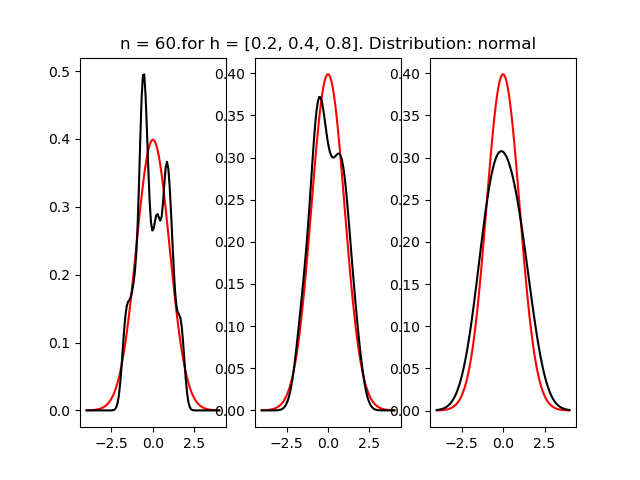
\includegraphics[width=\textwidth]{normalker60.png} 
			\caption[Нормальное распределение n = 60]{Нормальное распределение n = 60}
		\end{figure}
		\newpage
		\begin{figure}[h!]
			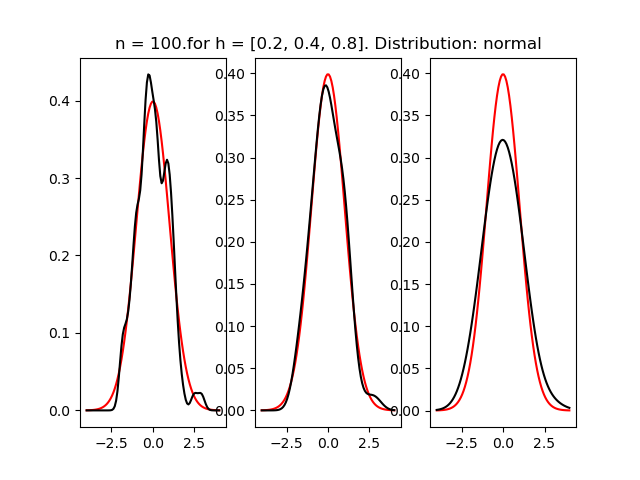
\includegraphics[width=\textwidth]{normalker100.png} 
			\caption[Нормальное распределение n = 100]{Нормальное распределение n = 100}
		\end{figure}
		\newpage
		\begin{figure}[h!]
			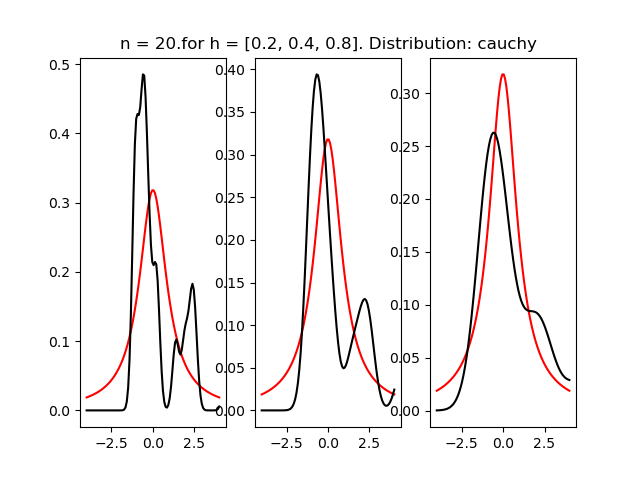
\includegraphics[width=\textwidth]{cauchyker20.png}
			\caption[Распределение Коши n = 20]{Распределение Коши n = 20}
		\end{figure}
		\newpage
		\begin{figure}[h!]
			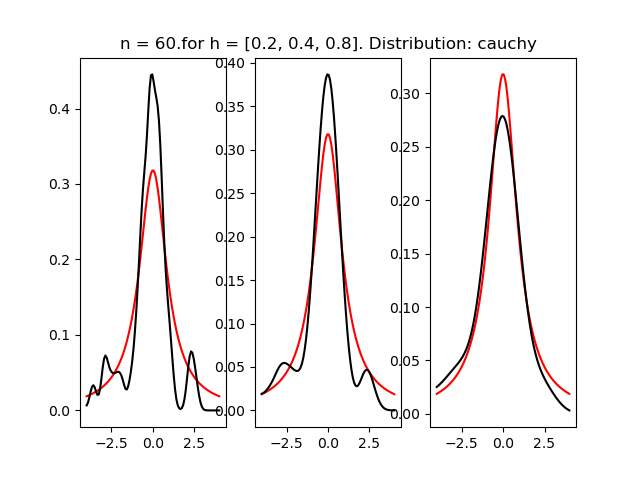
\includegraphics[width=\textwidth]{cauchyker60.png}
			\caption[Распределение Коши n = 60]{Распределение Кошиn = 60}
		\end{figure}
		\newpage
		\begin{figure}[h!]
			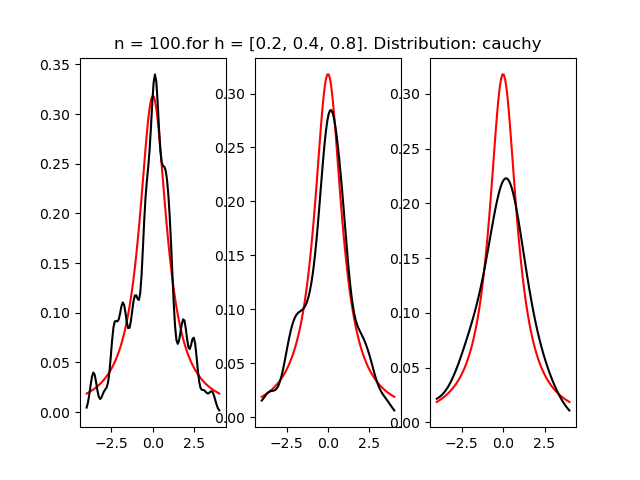
\includegraphics[width=\textwidth]{cauchyker100.png}
			\caption[Распределение Коши n = 100]{Распределение Коши n = 100}
		\end{figure}
		\newpage
		\begin{figure}[h!]
			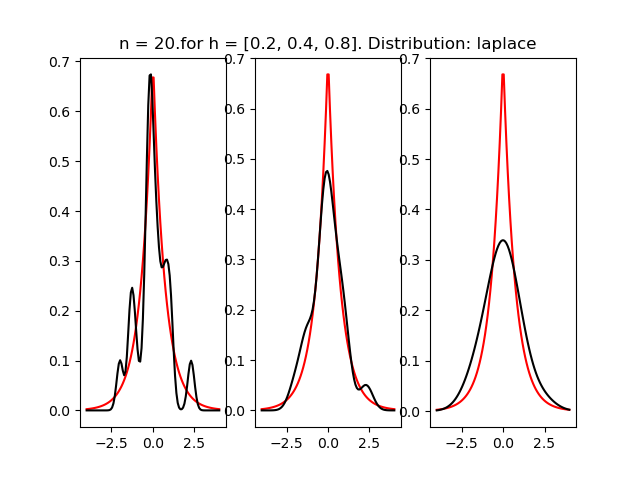
\includegraphics[width=\textwidth]{laplaceker20.png}
			\caption[Распределение Лапласа n = 20]{Распределение Лапласа n = 20}
		\end{figure}
		\newpage
		\begin{figure}[h!]
			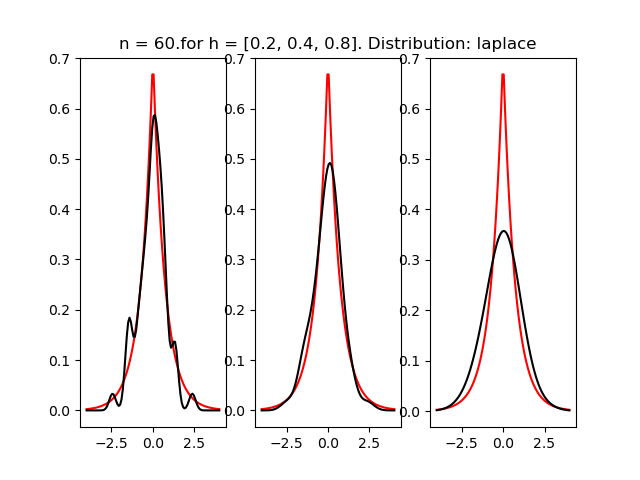
\includegraphics[width=\textwidth]{laplaceker60.png}
			\caption[Распределение Лапласа n = 60]{Распределение Лапласа n = 60}
		\end{figure}
		\newpage
		\begin{figure}[h!]
			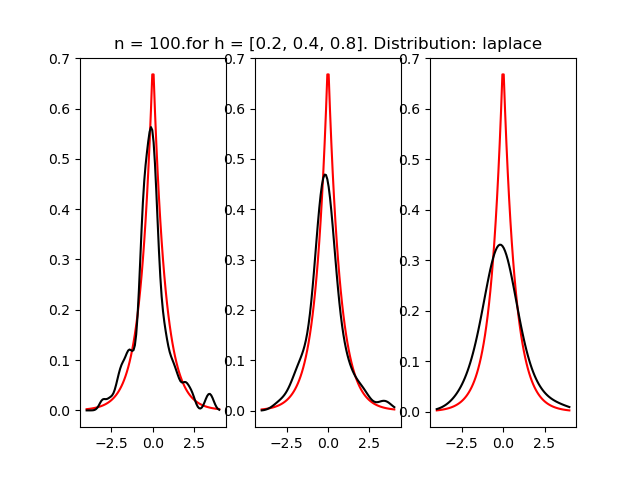
\includegraphics[width=\textwidth]{laplaceker100.png}
			\caption[Распределение Лапласа n = 100]{Распределение Лапласа n = 100}
		\end{figure}
		\newpage
		\begin{figure}[h!]
			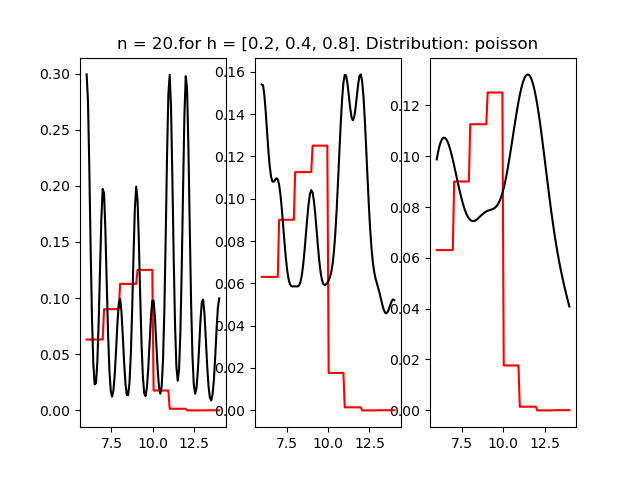
\includegraphics[width=\textwidth]{poissonker20.png}
			\caption[Распределение Пуассона n = 20]{Распределение Пуассона n = 20}
		\end{figure}
		\newpage
		\begin{figure}[h!]
			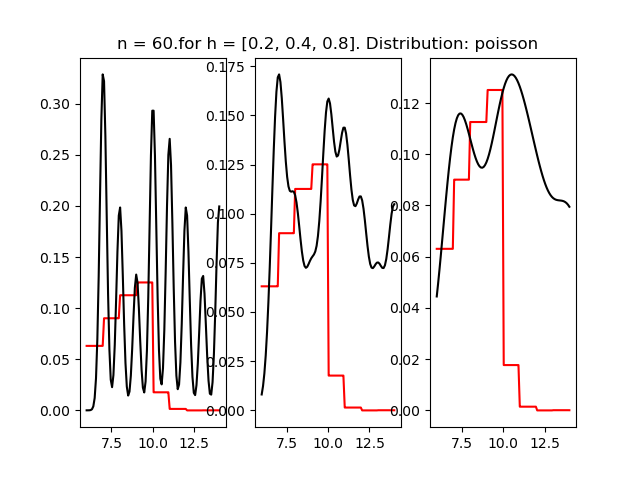
\includegraphics[width=\textwidth]{poissonker60.png}
			\caption[Распределение Пуассона n = 60]{Распределение Пуассона n = 60}
		\end{figure}
		\newpage
		\begin{figure}[h!]
			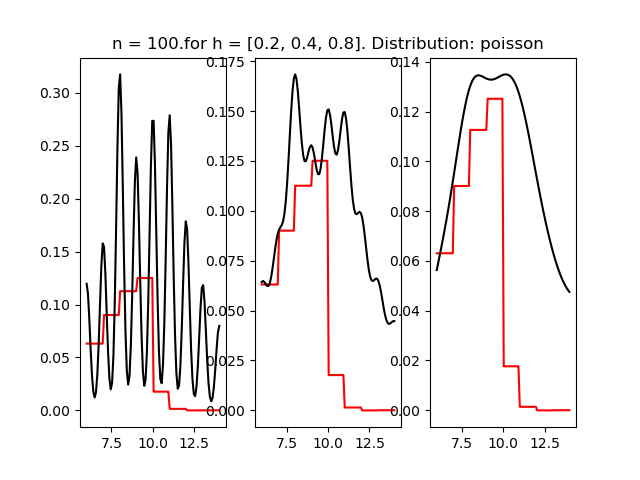
\includegraphics[width=\textwidth]{poissonker100.png}
			\caption[Распределение Пуассона n = 100]{Распределение Пуассона n = 100}
		\end{figure}
		\newpage
		\begin{figure}[h!]
			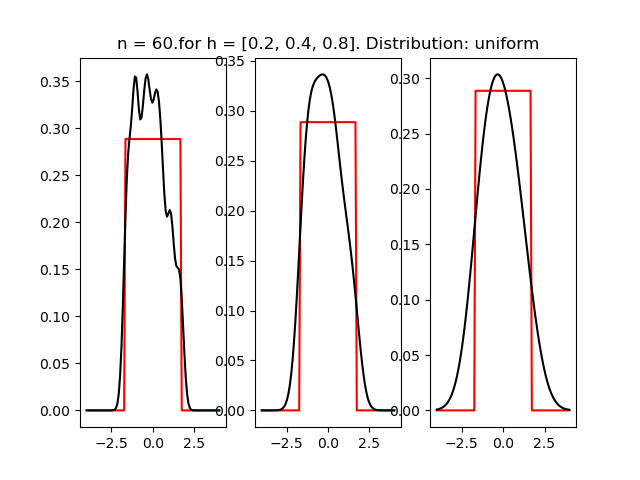
\includegraphics[width=\textwidth]{uniformker60.png}
			\caption[Равномерное распределение n = 60]{Равномерное распределение n = 60}
		\end{figure}
		\newpage
		\begin{figure}[h!]
			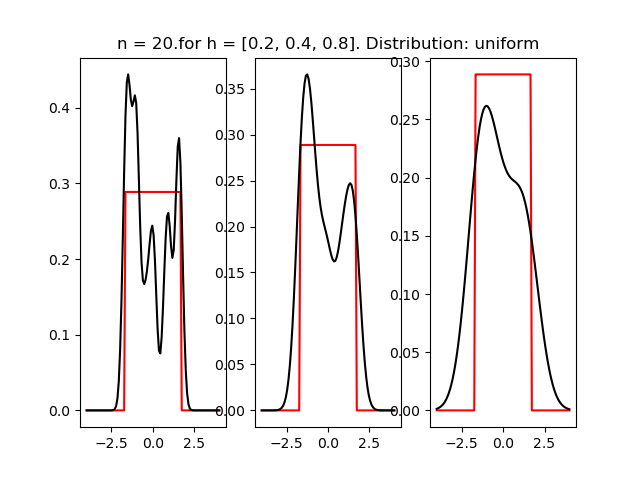
\includegraphics[width=\textwidth]{uniformker20.png}
			\caption[Равномерное распределение n = 20]{Равномерное распределение n = 20}
		\end{figure}
		\newpage
		\begin{figure}[h!]
			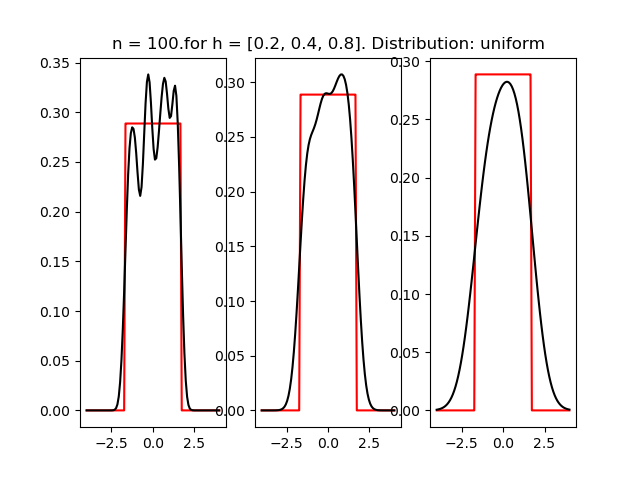
\includegraphics[width=\textwidth]{uniformker100.png}
			\caption[Равномерное распределение n = 100]{Равномерное распределение n = 100}
		\end{figure}
		
	\end{center}
		
	\newpage
	\section{Обсуждение}
		Видно, что эмпирическая функция лучше приближает эталонную функцию на больших выборках.\\
		
		При фиксированной ширине окна точнее приблизить функцию распределения позволяет увеличение выборки.\\
		
		Найлучшее приближение функции распределения ядерной функции для распределения Лапсласа, нормального распределения и распределения Коши достигается при $h =  h_n$, в свою очередь для равномерного распределения наилучшее приближение достигатеся при $ h = \frac{h_n}{2}$ и $h_n$. Для распределения Пуассона при $h = 2h_n$.
	
	\section{Литература}
	
	\href{https://physics.susu.ru/vorontsov/language/numpy.html}{Модуль numpy}\\
	
	\href{https://matplotlib.org/}{Модуль matplotlib}\\
	
	\href{https://www.scipy.org/}{Модуль scipy}\\
	
	\href{https://ru.wikipedia.org/wiki/%D0%AF%D0%B4%D0%B5%D1%80%D0%BD%D0%B0%D1%8F_%D0%BE%D1%86%D0%B5%D0%BD%D0%BA%D0%B0_%D0%BF%D0%BB%D0%BE%D1%82%D0%BD%D0%BE%D1%81%D1%82%D0%B8}{Ядерная оценки плотности}\\
	
	\section{Приложения}
	
	\href{https://github.com/LuciusGen/Matstat/blob/master/Lab4/Lab4.py}{Код лаборатрной}
	
	\href{https://github.com/LuciusGen/Matstat/blob/master/Lab4/lab4.tex}{Код отчёта}
	
\end{document}